\documentclass[a4paper,11pt,fleqn]{scrartcl}%fleqn pour aligner les equations à gauche
\usepackage{../../Styles/Cours}


\newcommand{\chnum}{Chapitre 09}
\newcommand{\chtitle}{Cohésion et dissolution des solides}
\newcommand{\dtype}{Cours}

\begin{document}
	\maketitle
\section{Structure et cohésion d'un solide ionique}
Un solide ionique ou cristal ionique est constitué de cations et d'anions dispersés de façon ordonnée dans l'espace. Il est électriquement neutre : les charges positives des cations sont compensées par les charges négatives des anions.\\
Sa formule, dite \textbf{formule statistique}, indique la nature et la proportion des ions présents sans en mentionner les charges.\\
\textit{ex. : \ce{CaF2(s)} contenant un ion calcium \ce{Ca^2+} et deux ions fluorure \ce{F-}}\\
Dans un cristal ionique, les ions exercent les ins sur les autres des forces d'interaction électrostatique soit attractive (entre deux ions de charge de signe opposés), soit répulsive (entre deux ions de charge de même signe). Cependant, chaque ion s'entoure d'ions de charges de signe contraires afin que les attractions s'emportent sur les répulsions.\\
\begin{cours}
    La \textbf{cohésion d'un cristal ionique} est assurée par les \textbf{intéractions ioniques}, c'est-à-dire par les \textbf{interactions électrostatiques} entre les ions de charges contraires du cristal. L'interaction ionique est une interaction \textbf{forte}.
\end{cours}

\section{Cohésion d'un solide moléculaire}
Un solide moléculaire est constitué de molécules. Il est cristallin si elles sont arrangées de façon ordonnée, sinon il est amorphe.\\
Leur cohésion est assurée par deyx types d'interactions électroqtatiques, plus faibles que celles qui assurent la cohésion des solides ioniques : les \textbf{interactions de van der Waals} et les \textbf{ponts hydrogène}.
    \subsection{Interactions de van der Waals}
    \begin{cours}
        Les interactions de \textbf{van der Waals} entre molécules sont :
        \begin{itemize}
            \item de type électrostatique
            \item attractives
            \item à courte portée ($< 10^{-9}$ m)
        \end{itemize}
    \end{cours}
    Ce sont des liaisons \textbf{intermoléculaires}, par opposition aux liaisons intramoléculaires  comme les liaisons covalentes qui s'établissent entre les atomes d'une même molécule.\\
    Ces interactions s'établissent entre les nuages électroniques des entités. Leurs valeurs de force sont faibles comparativement aux liaisons covalentes et aux liaisons ioniques et concernent les molécules polaires comme apolaires. Les interactions de van der Walls sont d'autant plus fortes que les électrons sont nombreux et que la molécules est volumineuse.\\
    On considère trois types de liaisons de van der Waals :
    \subsubsection{interaction entre les charges partielles de deux molécules polaires}
    \begin{minipage}{.58\linewidth}
                Les molécules \textbf{polaires s'orientent} de telle sorte que l'atome portant une charge partielle $\delta^+$ soit attiré par l'atome portant une charge partielle $\delta^-$\\
    Plus les molécules sont polaires et plus les interactions de van der Waals sont fortes.
            \end{minipage}\begin{minipage}{.38\linewidth}
                \centering
                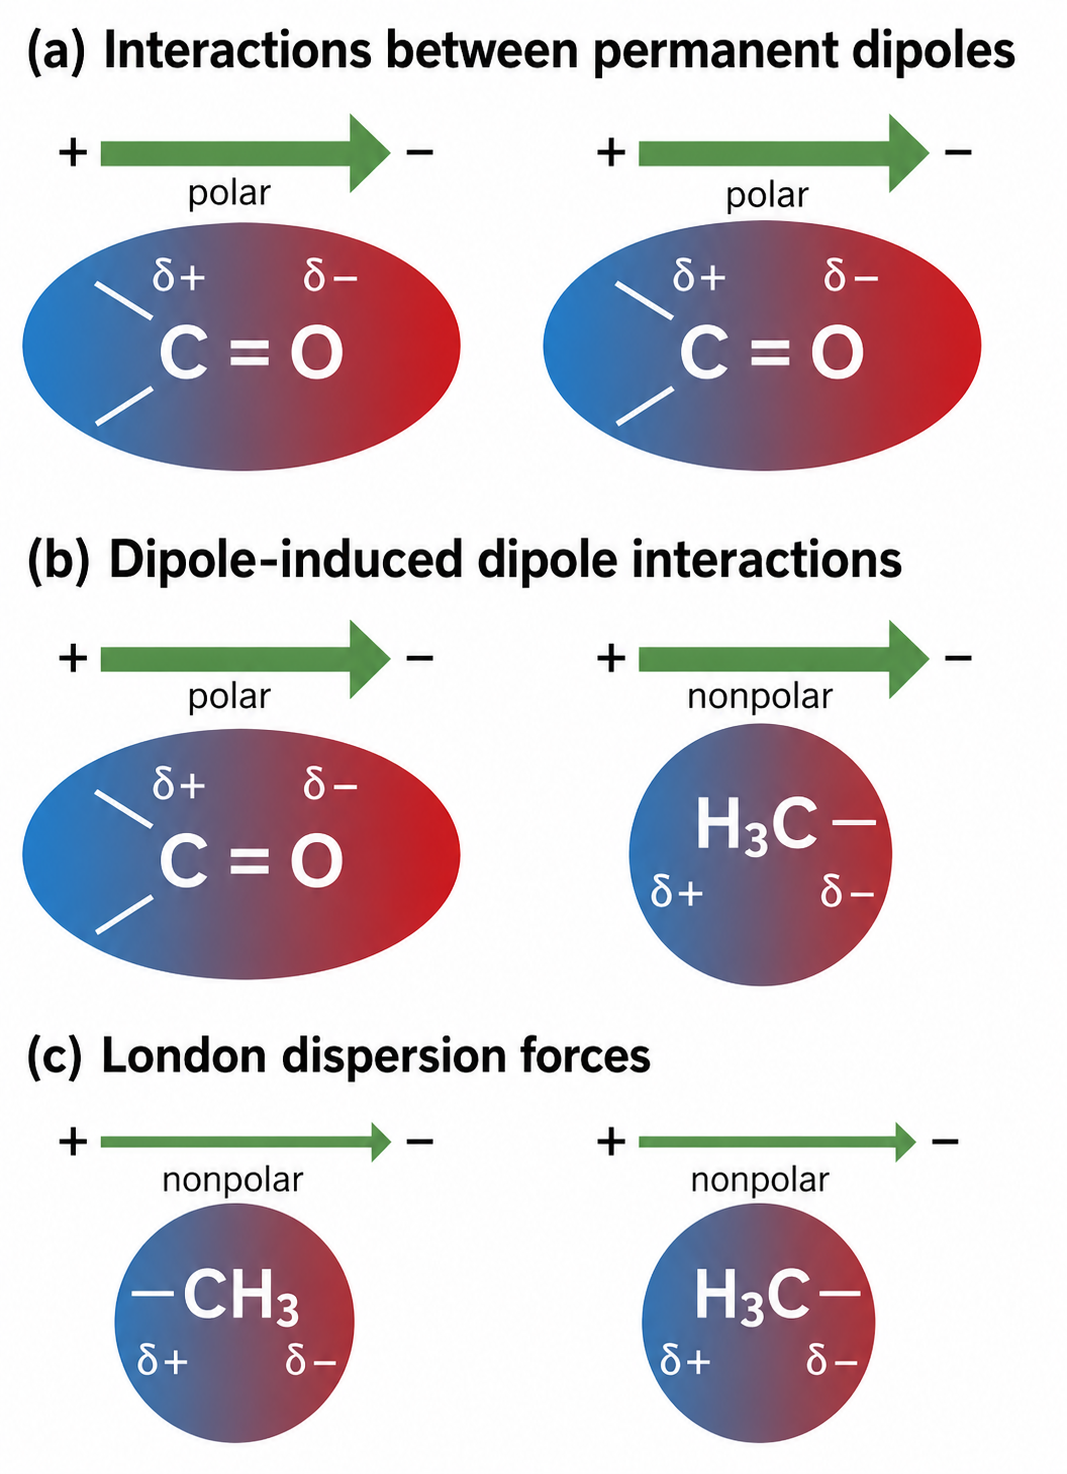
\includegraphics[trim={0 34cm 0 0},clip, width=\linewidth]{Ressources/vanderwaals_2.png}
            \end{minipage}
    

    \subsubsection{interaction entre une molécule polaire et une molécule apolaire}
    \begin{minipage}{.58\linewidth}
    Une molécule polaire peut \textit{induire} une déformation du nuage électronique d'une molécule apolaire voisine et ainsi la polariser temporairement par influence.\\
    Les interactions de van der Waals entre molécules polaires et apolaires sont plus faibles que celles entre deux molécules polaires. Elles sont d'autant plus intenses qu'elles s'établissent entre une molécule fortement polaire et une molécule apolaire fortement polarisable (donc de grande taille).
    \end{minipage}
    \begin{minipage}{.38\linewidth}
                \centering
                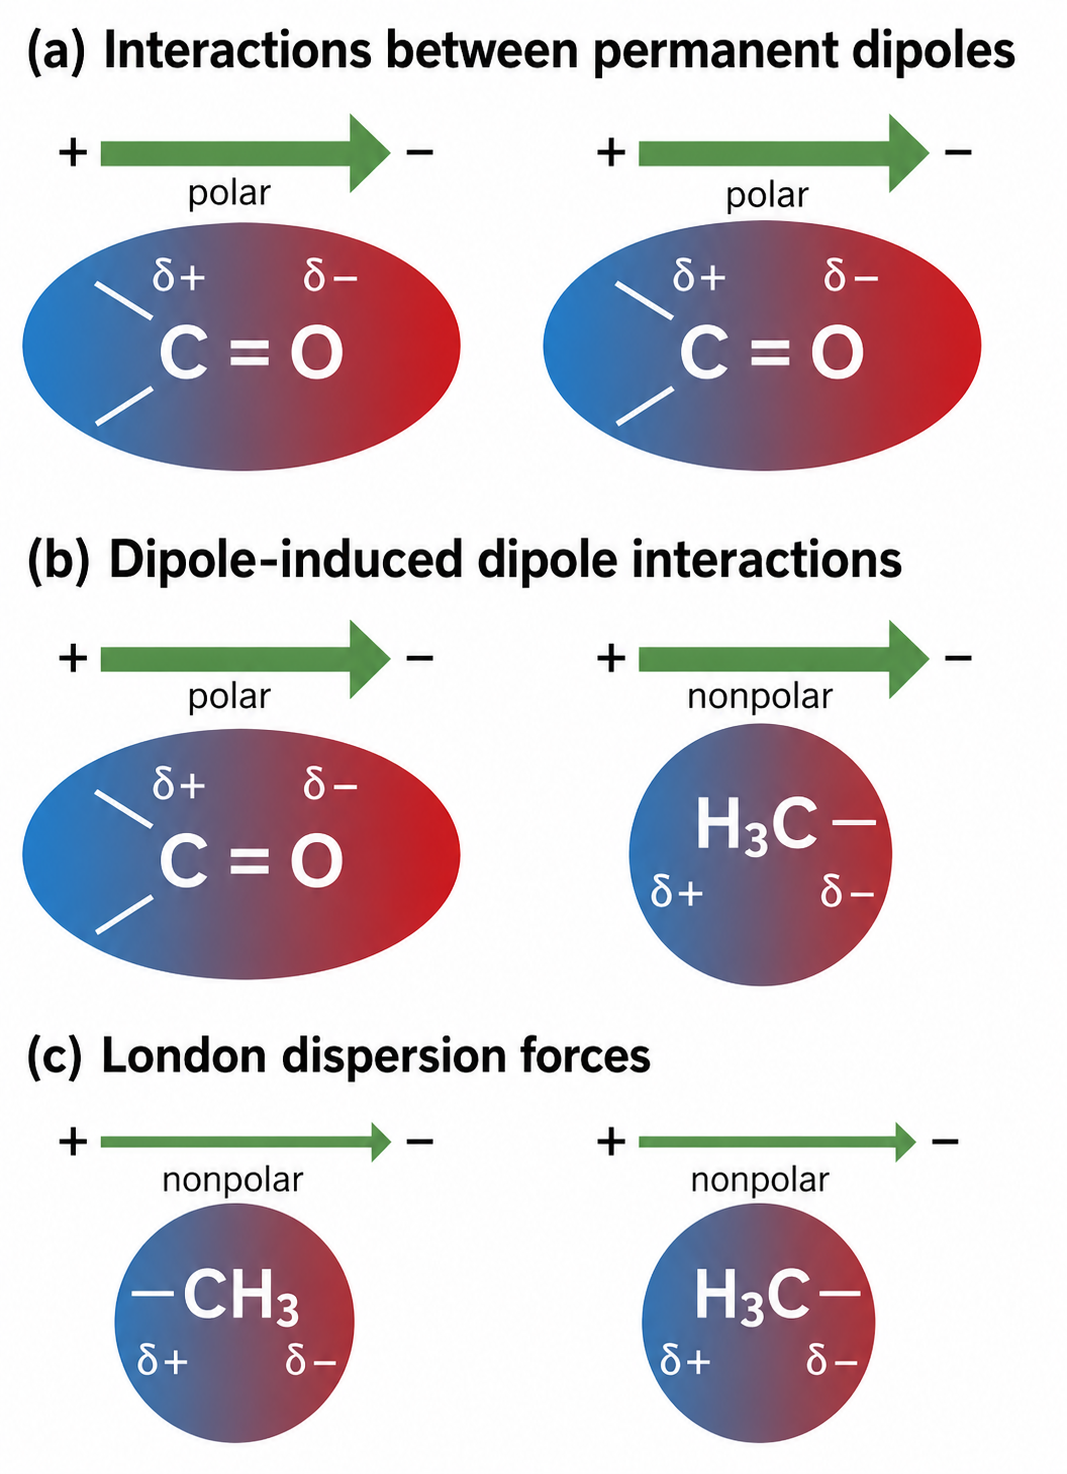
\includegraphics[trim={0 16cm 0 18cm},clip, width=\linewidth]{Ressources/vanderwaals_2.png}
            \end{minipage}
    \subsubsection{interaction entre deux molécules apolaires}
    \begin{minipage}{.58\linewidth}
    En raison du mouvement incessant des électrons dans une molécule, celle-ci présente à chaque instant une polarisation, bien que la polarisation dans le temps soit nulle. C'est pourquoi elle peut polariser par influence une molécule apolaire voisine.\\
    Les interactions de van der Waals entre deux espèces apolaires sont d'autant plus fortes que les espèces considérées sont polarisables.
     \end{minipage}
    \begin{minipage}{.38\linewidth}
                \centering
                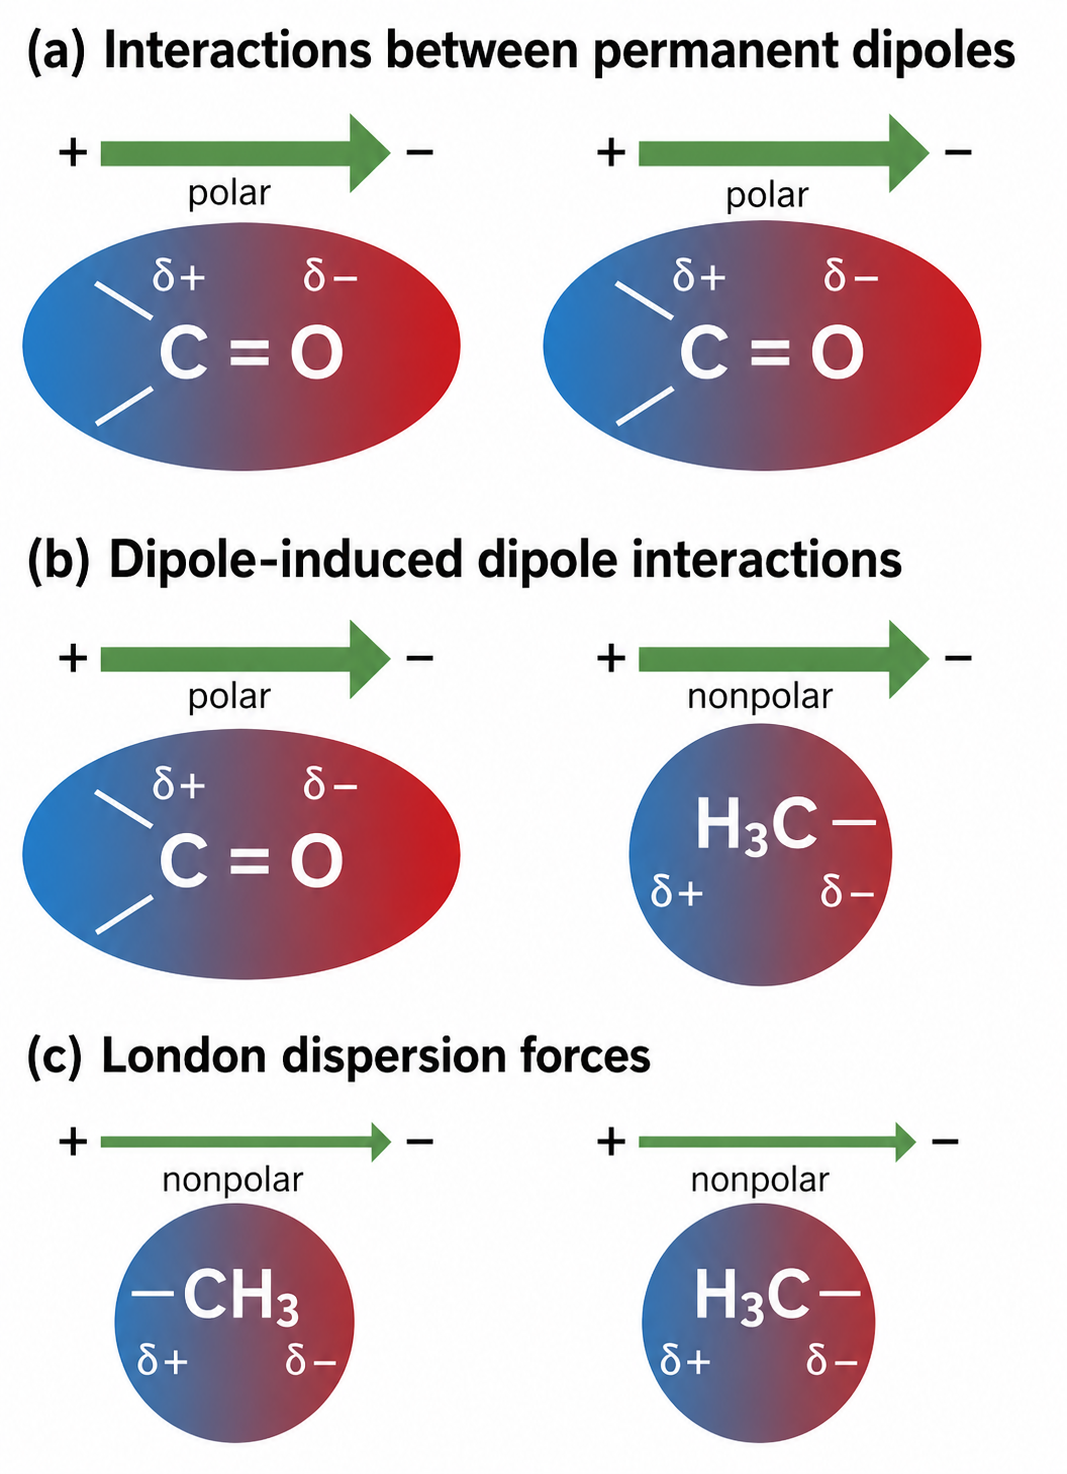
\includegraphics[trim={0 0 0 36cm},clip, width=\linewidth]{Ressources/vanderwaals_2.png}
            \end{minipage}

    Les interactions de van der Waals sont prépondérantes dans les molécules apolaires de tailles importantes et dans les molécules polaires.

    \subsection{Pont hydrogène}
    Un pont hydrogène peut s'établir entre des molécules identiques ou différentes (liaison intermoléculaire) ou entre atomes d'une même molécules (liaison intramoléculaire).\\
    Il correspond à une \textbf{interaction électrostatique attractive} qui s'établit entre une molécules possédant un \textbf{atome d'hydrogène} lié à un \textbf{atome de forte électronégativité} (liaisons O-H, N-H, F-H), et une autre molécule comportant une \textbf{atome électronégatif} (O, N, F) possédant au moins un doublet non liant.\\
    Le pont hydrogène est une interaction plus forte qu'une interaction de van der Waals et n'existe que si les atomes sont suffisament proches (séparés de \num{0,1} à \SI{5,0}{nm}). C'est ce type d'interaction qui maintien par exemple ensemble les deux brins de la molécule d'ADN.
    \begin{figure}[h!]
            \begin{minipage}{.48\linewidth}
                \centering
                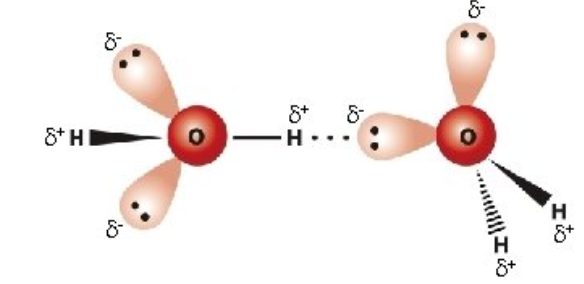
\includegraphics[width=.8\linewidth]{Ressources/HBound.PNG}
            \end{minipage}
            \begin{minipage}{.48\linewidth}
                \centering
                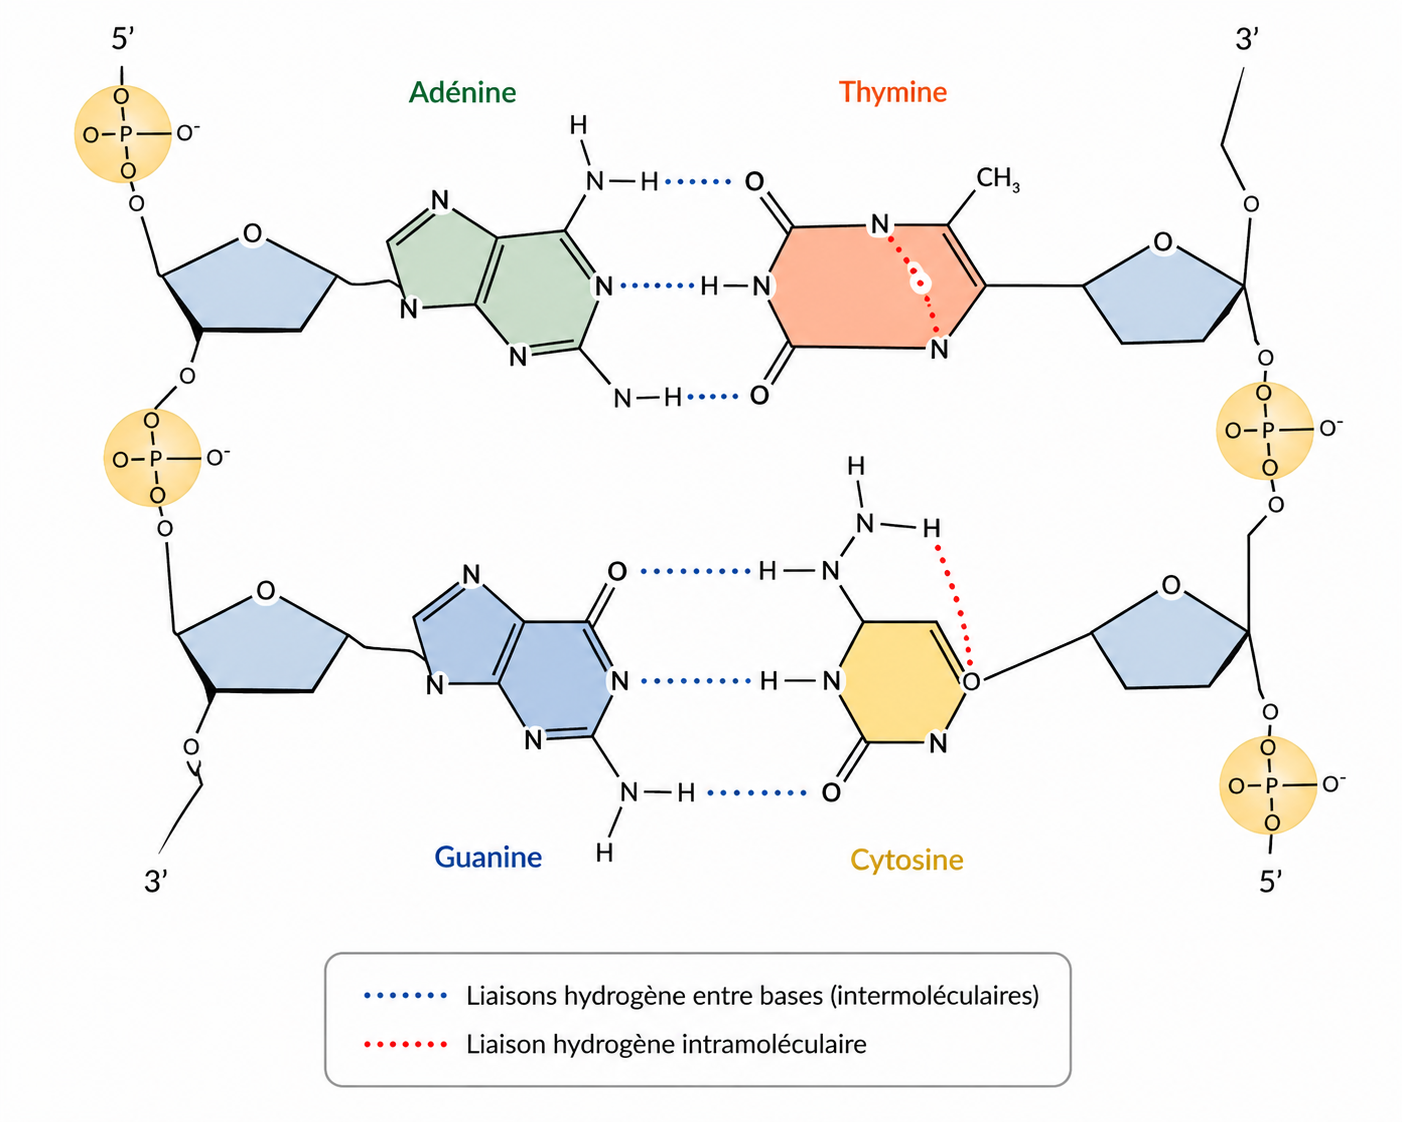
\includegraphics[width=\linewidth]{Ressources/ChatGPT Image Apr 29, 2026, 07_40_44 AM.png}
            \end{minipage}
           
        \end{figure}

        \newpage
    \subsection{Interaction intermoléculaire et propriétés physico-chimique}
    Les interactions intrémoléculaires lient les atomes dans une molécules et sont responsables de leur stabilité. Les interactions intermoléculaires sont responsables des propriétés physico-chimiques.\\
    Les températures de fusion et d'ébullition d'un corps pur sont élevées lorsque des interactions intermoléculaires nombreuses et intenses peuvent s'établir entre les molécules.\\
    Plus les molécules d'un soluté peuvent établir d'interactions avec les molécules d'un solvant, plus grande sera la solubilité de ce soluté, dans ce solvant. Il en est de même pour la miscibilité entre deux liquides.\\
    Les interactions ioniques sont plus fortes que les interactions intermoléculaires, il est donc nécessaire de fournir aux solides ionique davantage d'énergie thermique pour rompre ces interactions.\\
    \textit{Les températures de changements d'état des composés ioniques sont en général plus élevées que celles des corps purs moléculaires.}

    \section{Dissolution d'un solide ionique}
        \subsection{Processus de dissolution}
        La dissolution d'un solide ionique s'effectue en trois étapes : 
        \begin{enumerate}
            \item \textbf{Dissociation} : Sous l'effet des interactions électrostatiques s'exerçant entre l'eau (solvant) et les ions à la surface du cristal, celui-ci finit par se disocier.
            \item \textbf{Solvatation des ions libérés} : Les ions s'entourent de molécules d'eau et s'isolent les uns des autres. Les ions solvatés ou hydratés (dans le cas où le solvant est l'eau) sont notés avec les symbole (aq), par exemple \ce{Na+(aq)}.
            \item \textbf{Dispersion} : Sous l'effet de l'agitation thermique et selon la nature du solvant, les ions solvatés se dispsersent dans le solvant.
        \end{enumerate}
        \begin{figure}[t!]
            \centering
            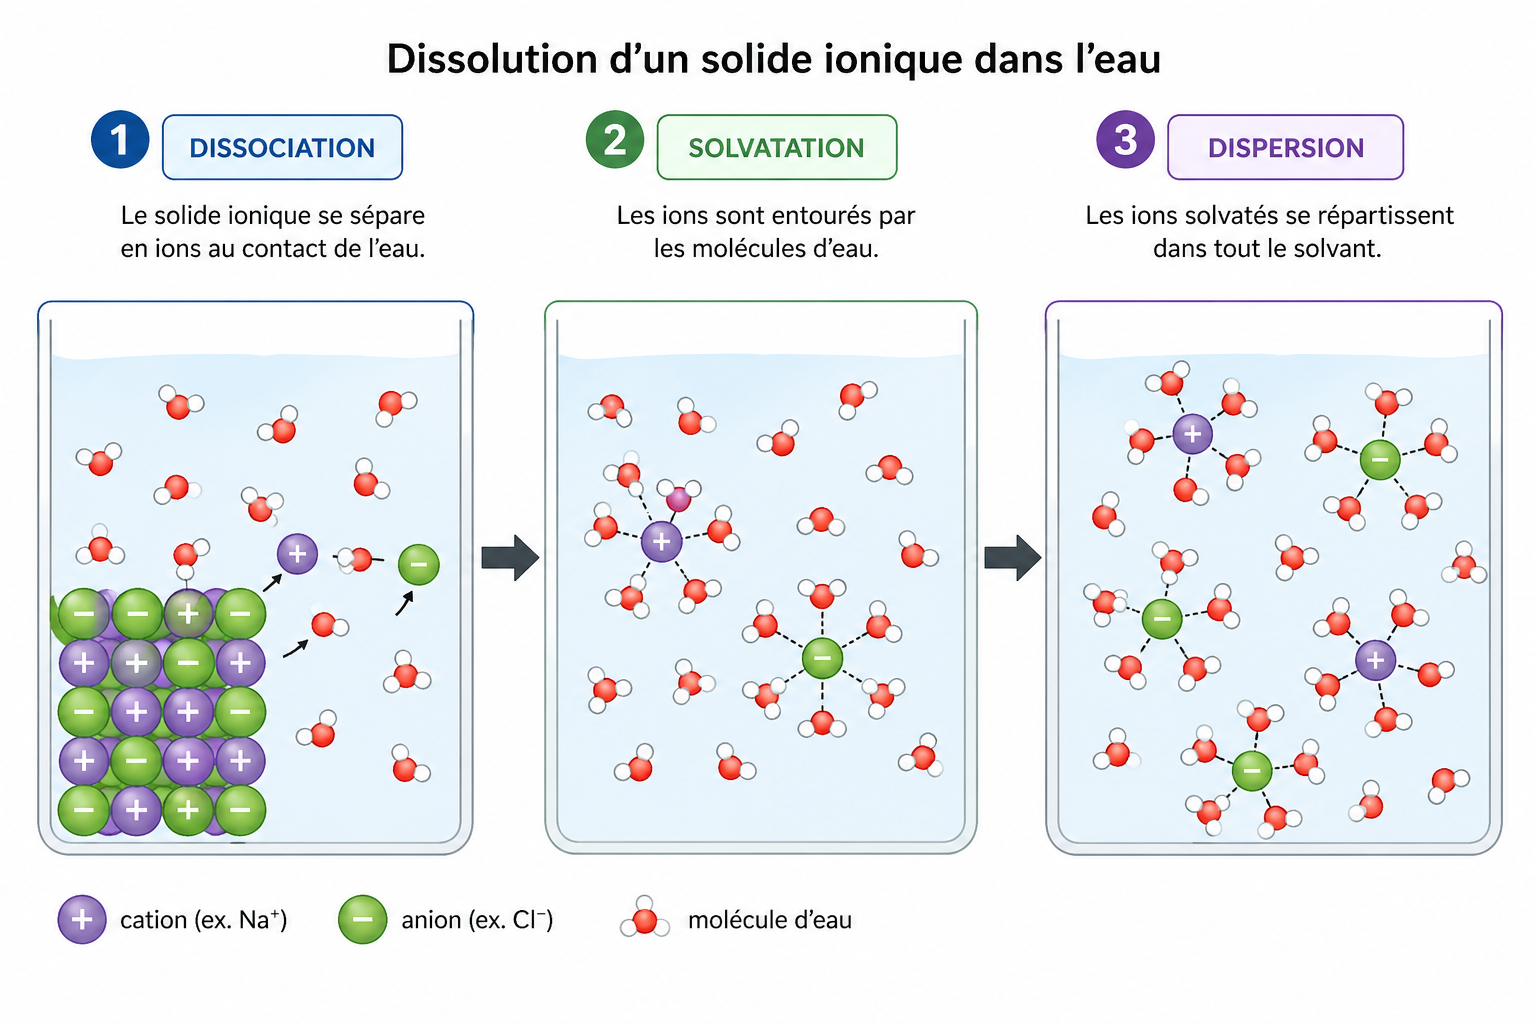
\includegraphics[width=.6\linewidth]{Ressources/ChatGPT Image Apr 29, 2026, 07_33_51 AM.png}
        \end{figure}

\end{document}